\documentclass[11pt]{article}

\usepackage{a4wide}
\usepackage[utf8]{inputenc}
\usepackage[russian]{babel}
\usepackage{graphicx}
\usepackage{amsmath}
\usepackage{amsthm}
\usepackage{amssymb}
\usepackage{enumitem}
\usepackage{mathtools}

\newtheorem{theorem}{Теорема}

\newcommand*{\hm}[1]{#1\nobreak\discretionary{}{\hbox{$\mathsurround=0pt #1$}}{}}
\newcommand\abs[1]{\left\lvert#1\right\rvert}
\newcommand{\scalar}[2]{\left<#1,#2\right>}

%\renewcommand{\theequation}{\textbf{(\arabic{equation})}}

\begin{document}
\thispagestyle{empty}

\begin{center}
\ \vspace{-3cm} \newline
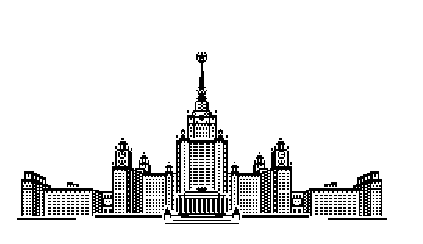
\includegraphics[width=0.5\textwidth]{msu.eps}\\
{\scshape Московский государственный университет имени М.~В.~Ломоносова}\\
Факультет вычислительной математики и кибернетики\\
Кафедра системного анализа

\vfill
{\LARGE Отчёт по практикуму} \\
%\vspace{1cm}
{\Huge\bfseries <<Переписывание>>}
\end{center}

\vspace{1cm}
\begin{flushright}
\large
\textit{Студент 315 группы}\\
В.~С.~Терёшин\\
%\vspace{5mm}
%\textit{Руководитель практикума}\\
%к.ф.-м.н., доцент П.~П.~Петров
\end{flushright}

\vfill
\begin{center}
Москва, 2013
\end{center}

\pagebreak
\newtagform{bold}[\textbf]{\textbf(}{\textbf)}
\usetagform{bold}

В силу формулы \textbf{(9.28)} имеем
$$
y' = \frac{1}{2a} \frac{x + a}{x - a} \left( \frac{x - a}{x + a} \right)' = \frac{1}{2a} \frac{x + a}{x - a} \frac{x + a - \left( x - a \right)}{\left( x + a \right)^2} = \frac{1}{x^2 - a^2}.
$$
\begin{enumerate}[label=\bfseries \arabic*.]
\setcounter{enumi}{3}
\item
Найдём производную функции $ y = \ln \abs{x + \sqrt{x ^ 2 + A}} $.
Аналогично предыдущему примеру получим
$$
y' = \frac{1}{x + \sqrt{x^2 + A}} \left( \sqrt{x^2 + A} \right)' \hm=
\frac{1}{x + \sqrt{x^2 + A}} \left( 1 + \frac{x}{\sqrt{x^2 + A}} \right) \hm= \frac{1}{\sqrt{x^2 + A}}.
$$
\item
Пусть $ y = \ln^2 \arcsin \tfrac{1}{x} $, $ x > 1 $. Найдём производную и дифференциал этой функции:
\begin{gather}
y' = \left( \ln^2 \arcsin 1 / x \right) = 2 \ln \arcsin \dfrac{1}{x} \left( \ln \arcsin 1 / x \right)' = \notag \\
= 2 \ln \arcsin \dfrac{1}{x} \dfrac{1}{\arcsin 1 / x} \left( \arcsin 1 / x \right)' \hm= \notag \\
= 2 \dfrac{\ln \arcsin 1 / x}{\arcsin 1 / x} \dfrac{1}{\sqrt{1 - 1 / x^2}} \left( \dfrac{1}{x}\right)' = -\dfrac{2 \ln \arcsin 1 / x}{\abs{x} \sqrt{x^2 - 1} \arcsin 1 / x}. \notag
\end{gather}
Отсюда дифференциал находится непосредственно по формуле $ dy = y' dx $; однако если бы мы ещё не имели готового выражения для производной, то дифференциал можно было бы найти и непосредственно, используя его инвариантность относительно выбора переменных:
\begin{gather}
d \left( \ln^2 \arcsin 1 / x \right) = 2 \ln \arcsin 1 / x \, d \left( \ln \arcsin 1 / x \right) = \notag \\
= 2 \ln \arcsin \frac{1}{x} \frac{1}{\arcsin 1 / x} d \left( 1 / x \right) = \notag \\
= \frac{2 \ln \arcsin 1 / x}{\arcsin 1 / x}	\frac{1}{\sqrt{1 - 1 / x^2}} d \left( \frac{1}{x} \right) = \frac{-2 \ln \arcsin 1 / x}{\abs{x} \sqrt{x^2 - 1} \arcsin 1 / x} dx. \notag
\end{gather}
\item
Выведем с помощью теоремы 5 ещё одну часто применяемую формулу. Пусть $ y = u^v $, где $ u = u(x) > 0 $, $ v = v(x) $. Представим данную функцию в виде $ y = e^{v \ln u} $ и вычислим $ \tfrac{dy}{dx} $:
\begin{gather}
\dfrac{dy}{dx} = \dfrac{de^{v \ln u}}{dx} = e^{v \ln u} \dfrac{d}{dx} \left( v \ln u \right) = u^v \left( \dfrac{dv}{dx} \ln u + \dfrac{v}{u} \dfrac{du}{dx} \right) = \notag \\
= u^v \dfrac{dv}{dx} \ln u + vu^{v - 1} \dfrac{du}{dx}. \tag{9.29}
\end{gather}
\end{enumerate}
\end{document}
